% individual, feito no site da biblioteca central
% ver pagina 26 da MDT

\addtocounter{page}{-1}
\begin{fichacatalografica}
%O presente trabalho foi realizado com apoio da Coordenação de Aperfeiçoamento de Pessoal de Nível Superior - Brasil (CAPES) - Código de Financiamento 001
%\vspace*{\fill}
%\begin{figure}[h!]
%\centering
%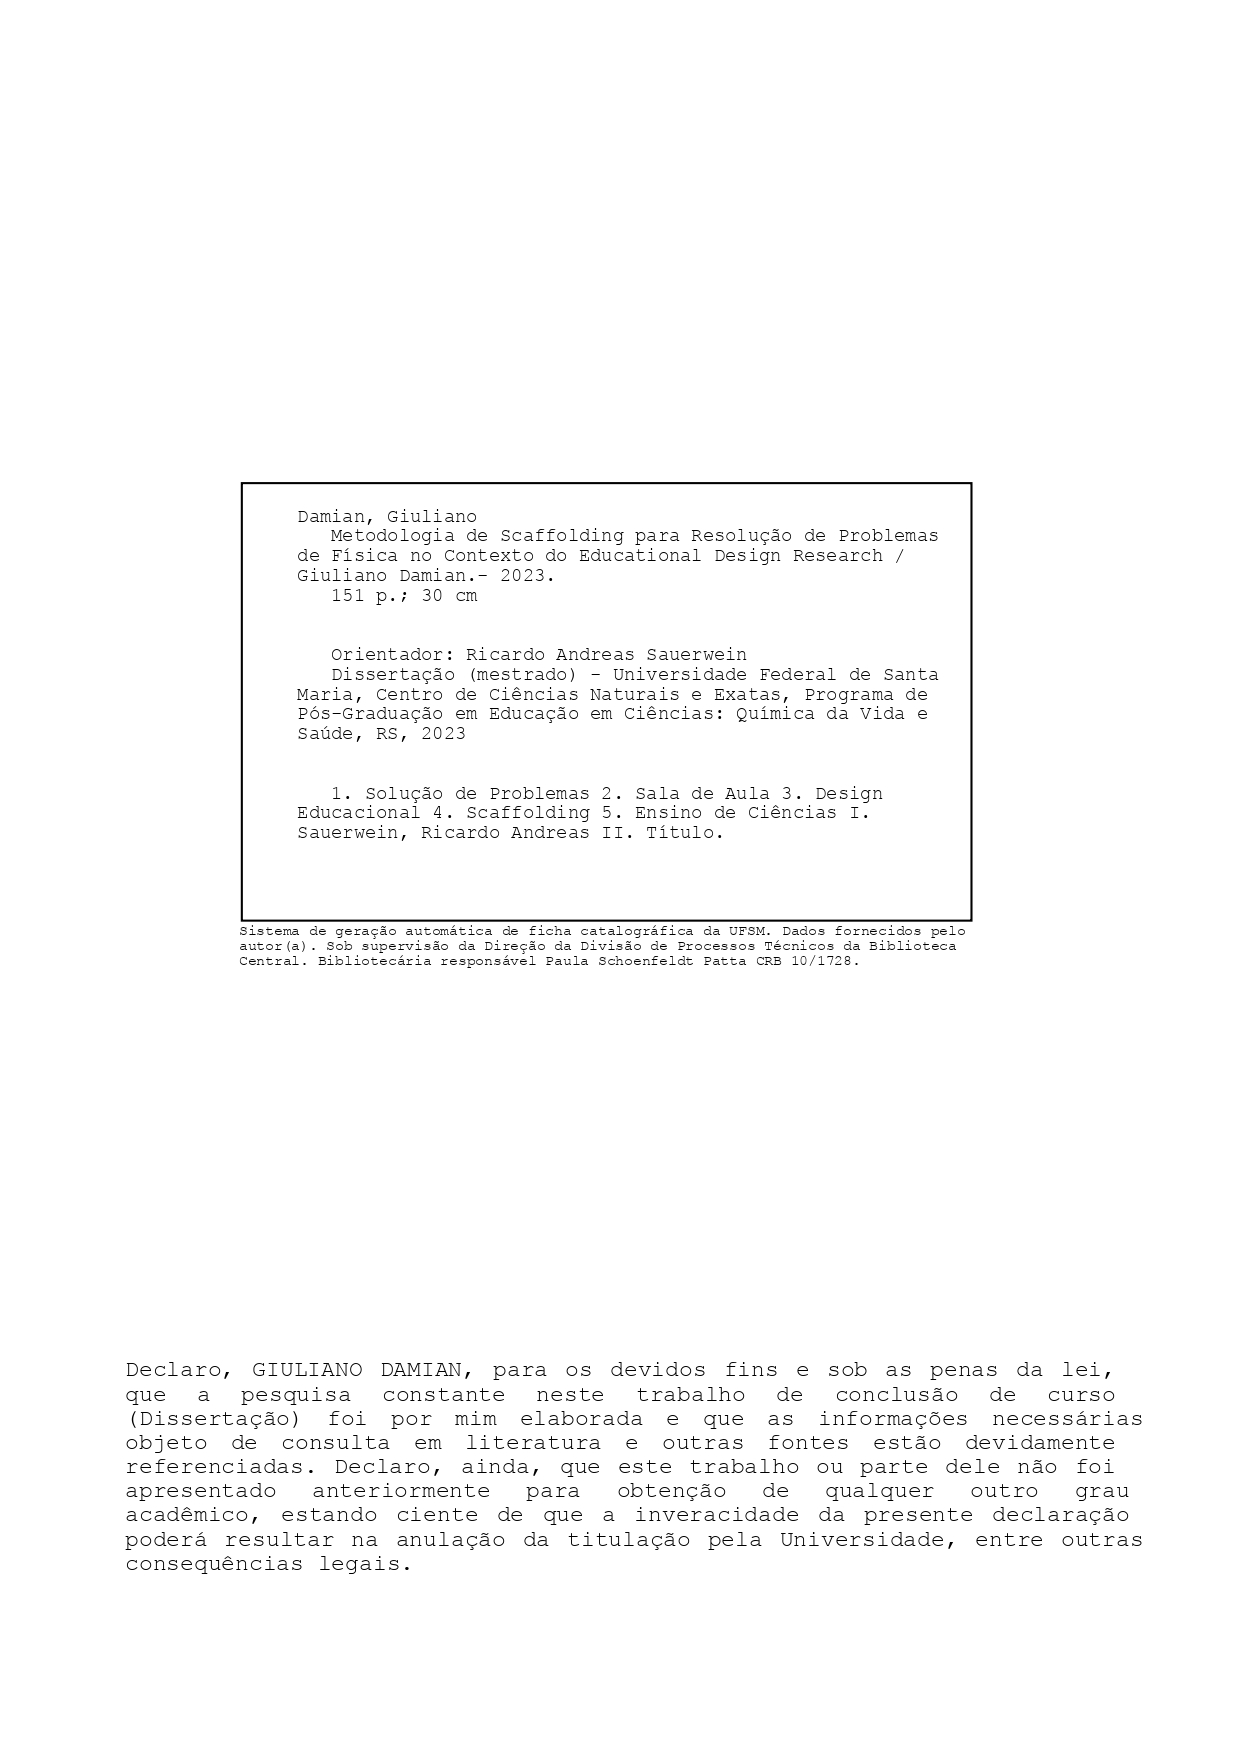
\includegraphics[width=\textwidth,height=\textheight,keepaspectratio]{fig/fichaCatalografica_page-0001.jpg}
%\end{figure}
%\noindent 2023\\
%Todos os direitos autorais reservados a \imprimirautor. A reprodução de partes ou do todo deste trabalho só poderá ser feita mediante a citação da fonte.\\
%E-mail: fsc.damian@gmail.com
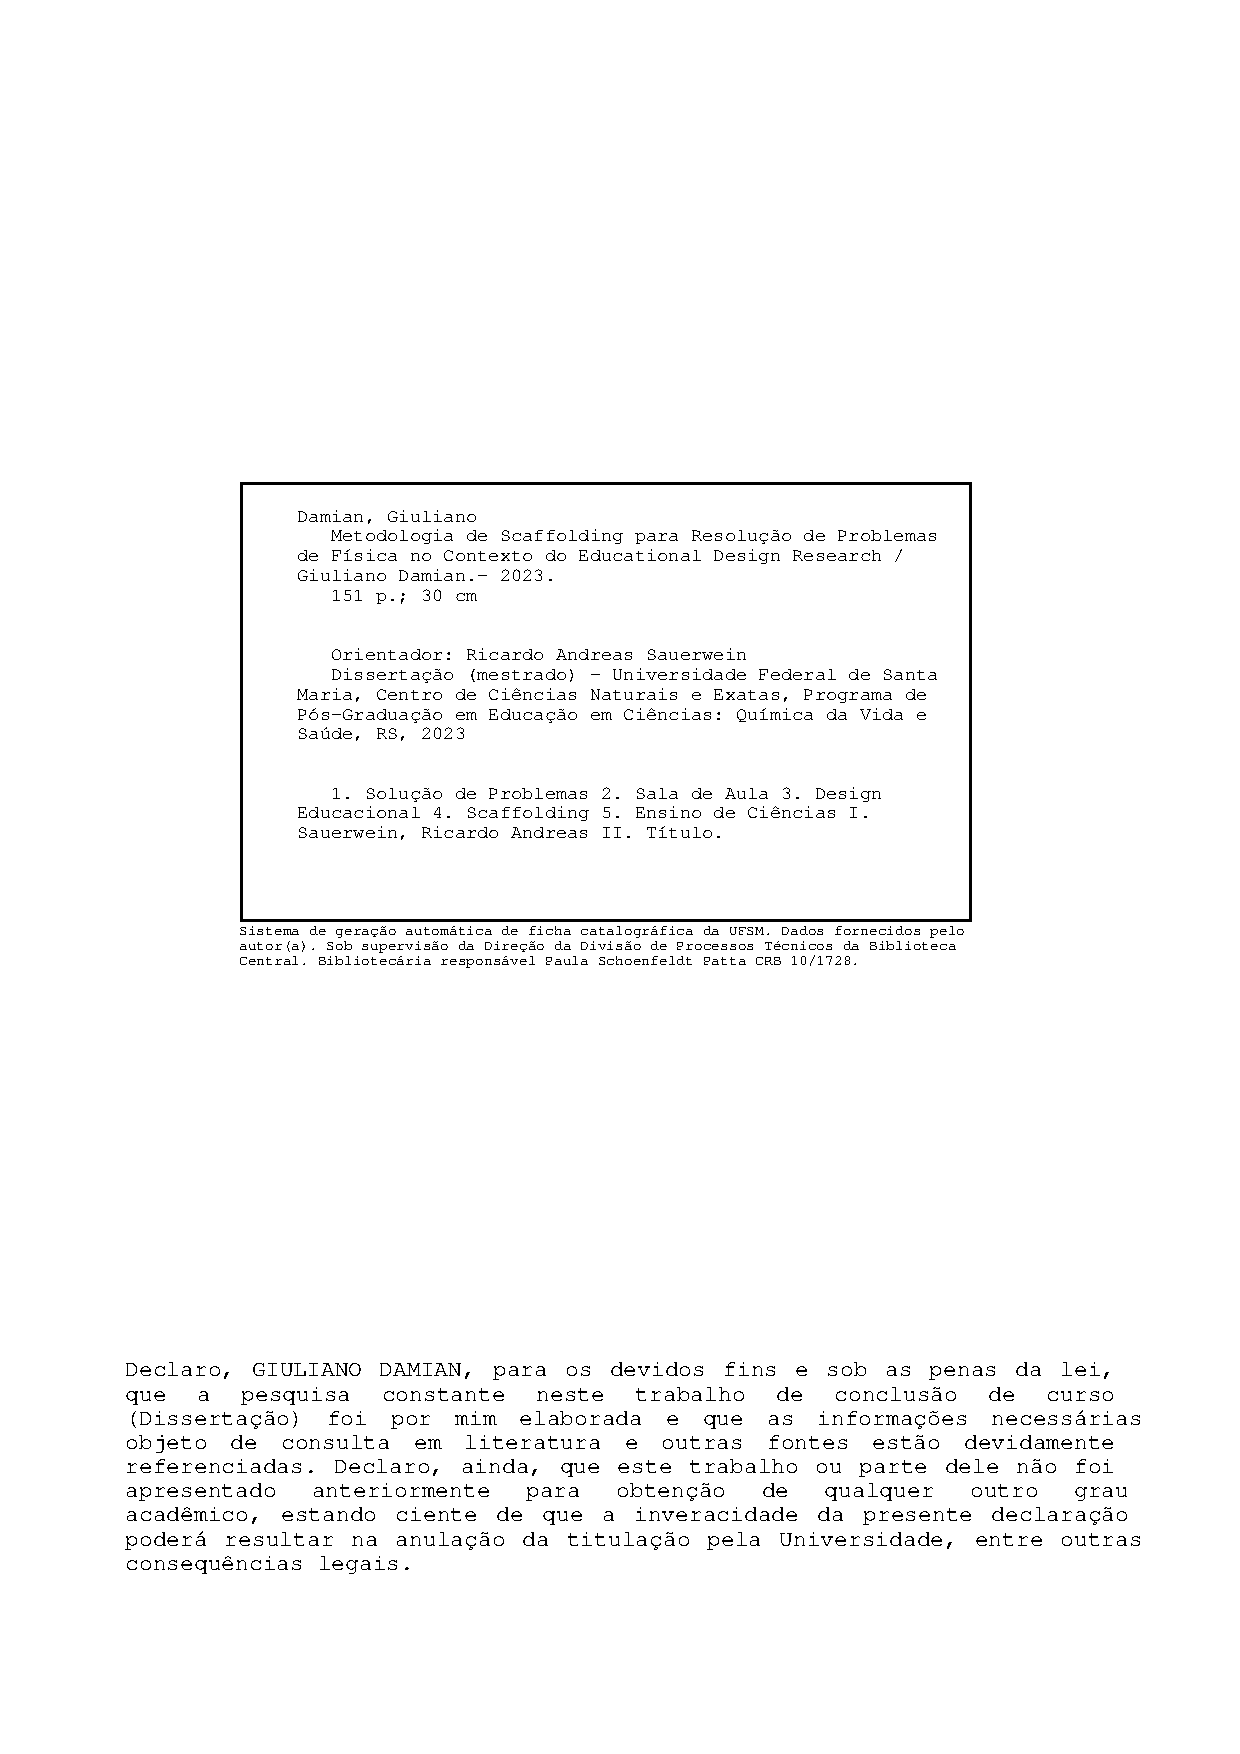
\includepdf[pages=-]{fig/fichaCatalografica.pdf}

\end{fichacatalografica}

% ATENÇÃO!
% Visando atender à exigência da CAPES, conforme Portaria nº 206, de 4 de setembro de
% 2018, 8 deve ser incluída a seguinte nota:
% O presente trabalho foi realizado com apoio da Coordenação de Aperfeiçoamento de Pessoal
% de Nível Superior - Brasil (CAPES) - Código de Financiamento 001
% This study was financed in part by the Coordenação de Aperfeiçoamento de Pessoal de Nível
% Superior - Brasil (CAPES) - Finance Code 001
